\documentclass[final]{siamltex}

% for red MarginPars
\usepackage{color}

% for \boldsymbol
\usepackage{amsmath}
\usepackage{latexsym}
\usepackage{graphicx}
\usepackage{geometry}
\usepackage{hyperref}

% total number of floats allowed on a page
\setcounter{totalnumber}{100}

% float page fractions
\renewcommand{\topfraction}{0.9}
\renewcommand{\bottomfraction}{0.9}
\renewcommand{\textfraction}{0.2}

% MarginPar
\setlength{\marginparwidth}{0.75in}
\newcommand{\MarginPar}[1]{\marginpar{\vskip-\baselineskip\raggedright\tiny\sffamily\hrule\smallskip{\color{red}#1}\par\smallskip\hrule}}

% for non-stacked fractions
\newcommand{\sfrac}[2]{\mathchoice
  {\kern0em\raise.5ex\hbox{\the\scriptfont0 #1}\kern-.15em/
   \kern-.15em\lower.25ex\hbox{\the\scriptfont0 #2}}
  {\kern0em\raise.5ex\hbox{\the\scriptfont0 #1}\kern-.15em/
   \kern-.15em\lower.25ex\hbox{\the\scriptfont0 #2}}
  {\kern0em\raise.5ex\hbox{\the\scriptscriptfont0 #1}\kern-.2em/
   \kern-.15em\lower.25ex\hbox{\the\scriptscriptfont0 #2}}
  {#1\!/#2}}

\def\Ab {{\bf A}}
\def\bb {{\bf b}}
\def\Fb {{\bf F}}
\def\gb {{\bf g}}
\def\Pb {{\bf P}}
\def\rb {{\bf r}}
\def\vb {{\bf v}}
\def\Wb {{\bf W}}
\def\xb {{\bf x}}

\def\deltab {\boldsymbol{\delta}}
\def\Psib   {\boldsymbol{\Psi}}
\def\Sigmab {\boldsymbol{\Sigma}}
\def\taub   {\boldsymbol{\tau}}

\def\half   {\frac{1}{2}}
\def\myhalf {\sfrac{1}{2}}

\begin{document}

%==========================================================================
% Title
%==========================================================================
\title{Implicit Low Mach Number Binary Mixing Notes}

\maketitle

\section{Introduction}
We have developed a new staggered grid code library for solving PDEs where scalars
are naturally cell-centered, and momentum and velocities are naturally face-centered,
or ``staggered'' in a MAC-stencil sense (see Figure \ref{fig:grid}).  We currently
have two applications: (i) a GMRES solver and (ii) an implicit low Mach number binary 
mixing code, which uses the GMRES solver.  In these notes we describe the implicit
low Mach number binary mixing code.  The GMRES solver is discussed in full detail 
in a forthcoming paper.  Within the code we also have an explicit binary mixing code,
but it is mostly self-contained and ideas from this code were used to develop the
low Mach number source code.
%%%%%%%%%%%%%%%%%%%%%%%%%%%%%%%%%
\begin{figure}[hb]
\centering
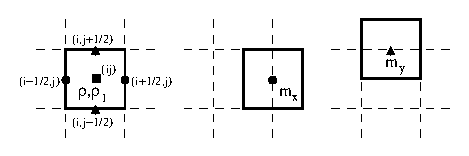
\includegraphics[width=5in]{grid}
\label{fig:grid}
\caption{Cartesian grid, finite volume grid structure with ``cell-centered'' scalars
and staggered momenta.}
\end{figure}
%%%%%%%%%%%%%%%%%%%%%%%%%%%%%%%%%

\section{Code Structure}
See Figure \ref{fig:flowchart} for a code structure chart.  Here is a summary
of what is contained within these directories:\\
%%%%%%%%%%%%%%%%%%%%%%%%%%%%%%%%%
\begin{figure}[tb]
\centering
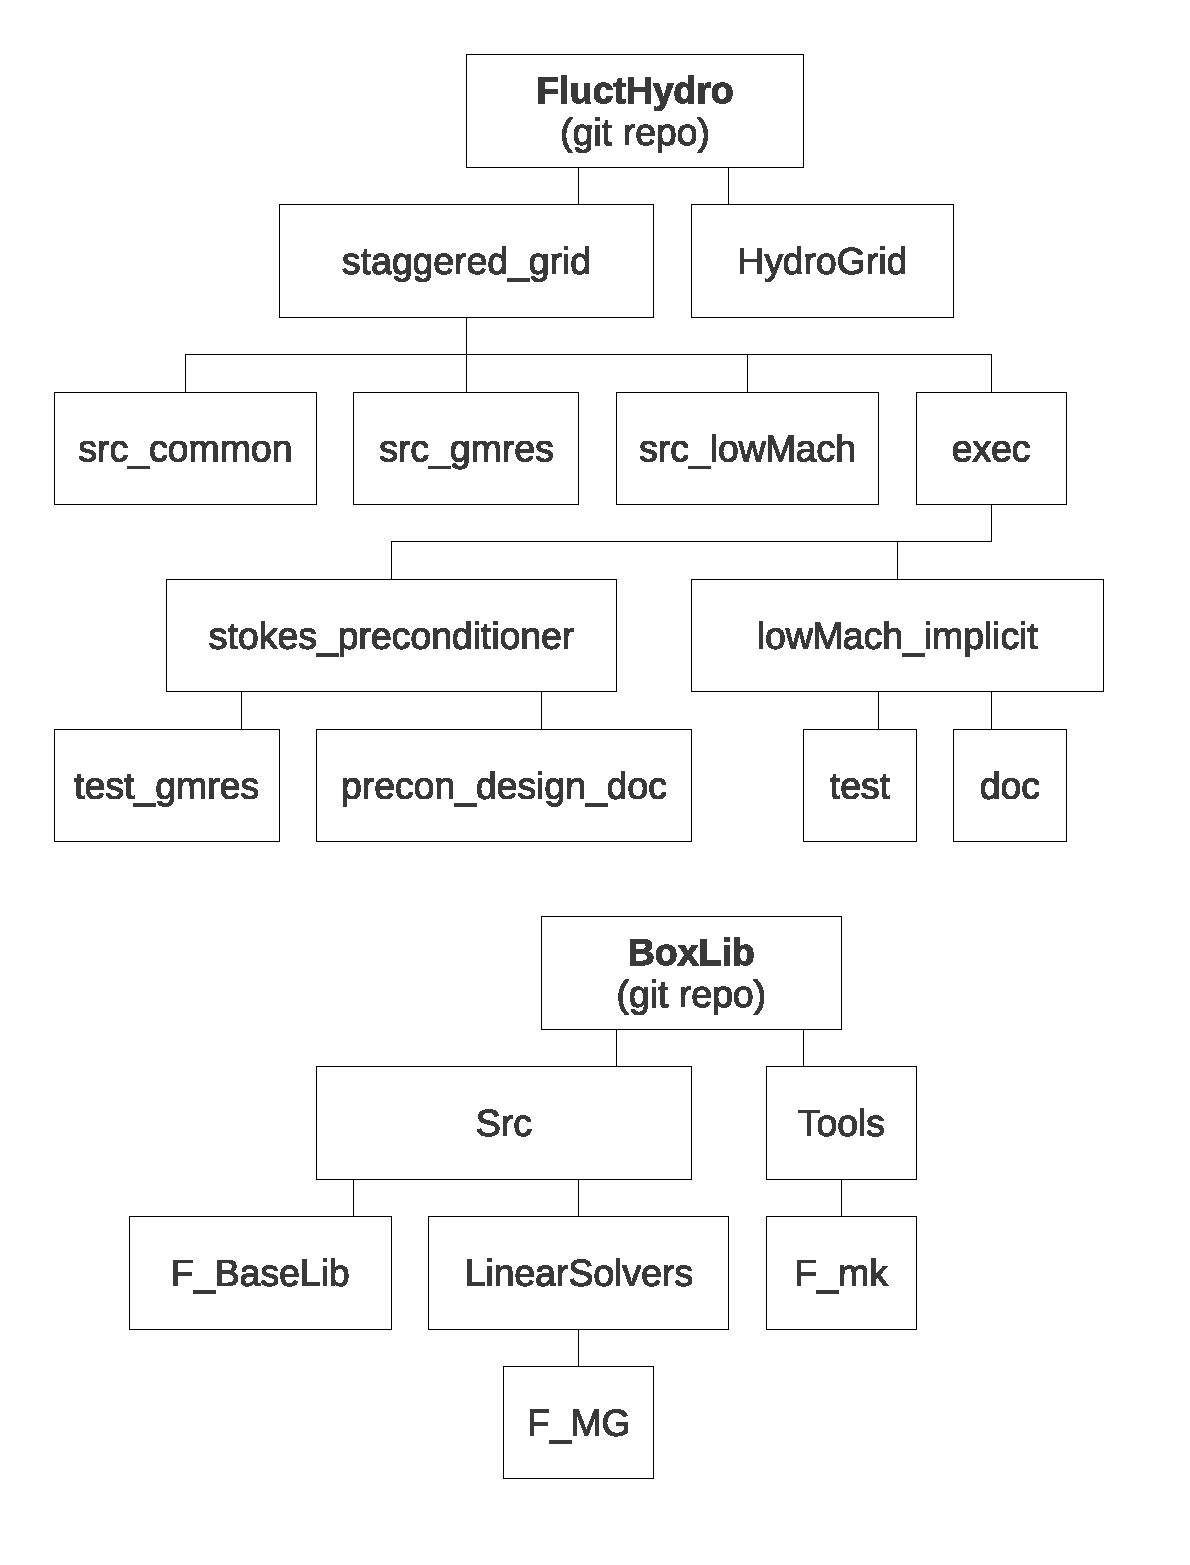
\includegraphics[width=3in]{flowchart}
\caption{Code structure chart for the source code for our staggered grid applications.}\label{fig:flowchart}
\end{figure}
%%%%%%%%%%%%%%%%%%%%%%%%%%%%%%%%%
\begin{itemize}
\item {\tt FluctHydro}\\
Git repo for all fluctuating hydrodynamics applications.
\begin{itemize}
\item {\tt staggered\_grid}\\
Staggered grid source code.
\begin{itemize}
\item {\tt src\_common}\\
Stuff that is common to all staggered grid codes.
\item {\tt src\_gmres}\\
Stuff required for the GMRES solver.
\item {\tt src\_lowMach}\\
Stuff required for any low Mach number time-advancement codes.
\item {\tt exec}\\
Stores all the run directories.
\begin{itemize}
\item {\tt stokes\_preconditioner}\\
Source code for the GMRES test code.
\item {\tt lowMach\_implicit}\\
Source code for the low Mach number implicit code.
\end{itemize}
\end{itemize}
\item {\tt HydroGrid}\\
Source code for random number generators and some analysis codes.
\end{itemize}
\item {\tt BoxLib}\\
Git repo for all BoxLib applications.
\begin{itemize}
\item {\tt Src}\\
BoxLib source code.
\begin{itemize}
\item {\tt F\_BaseLib}\\
Fortran90 BoxLib source code.
\item {\tt LinearSolvers}\\
Linear solver source code.
\begin{itemize}
\item {\tt F\_MG}\\
Fortran linear solver source code.  We use the cell-centered multigrid solver.
\end{itemize}
\end{itemize}
\item {\tt Tools}\\
BoxLib utilities.
\begin{itemize}
\item {\tt F\_mk}\\
Contains make system for Fortran90 BoxLib applications.
\end{itemize}
\end{itemize}
\end{itemize}

\section{Low Mach Number Binary Mixing Equations}
We have two incompressible fluids with densities $\bar\rho_1$ and $\bar\rho_2$, where 
each fluid does not change volume upon mixing.  Defining $\rho$ to be the density of
a mixture of these fluids, the densities of each fluid are $\rho_1 \equiv \rho c$ and 
$\rho_2 \equiv \rho(1-c)$, where $c$ is the {\it mass} fraction of the first fluid.  
Thus, $\rho = \rho_1 + \rho_2$.  Since the fluids do not change volume upon mixing, 
the equation of state will enforce that the {\it volume} fractions must sum to 1:
\begin{equation}
\frac{\rho_1}{\bar\rho_1} + \frac{\rho_2}{\bar\rho_2} =
\frac{\rho c}{\bar\rho_1} + \frac{\rho(1-c)}{\bar\rho_2} = 1 
\quad \rightarrow \quad
\rho = \left(\frac{c}{\bar\rho_1} + \frac{1-c}{\bar\rho_2}\right)^{-1}.
\end{equation}
The isothermal low Mach number equations of motion are:
\begin{eqnarray}
\partial_t\rho &=& -\nabla\cdot(\rho\vb),\\
\partial_t\rho_1 &=& -\nabla\cdot(\rho_1\vb) + \underbrace{\nabla\cdot\rho\chi\left(\nabla c + K_p\nabla p_0\right) + \nabla\cdot\Psib}_{\nabla\cdot\Fb},\\
\partial_t(\rho\vb) &=& -\nabla\cdot(\rho\vb\vb^T) - \nabla p + \nabla\cdot\taub(\vb) + \nabla\cdot\Sigmab + \rho\gb,
\end{eqnarray}
subject to
\begin{equation}
\nabla\cdot\vb = S \equiv \underbrace{\left(\frac{1}{\bar\rho_1}-\frac{1}{\bar\rho_2}\right)}_{-\beta/\rho}\nabla\cdot\Fb.
\end{equation}
Thus, $S \equiv S(\Fb)$.  The baro-diffusion coefficient is given by
\begin{equation}
K_P = \frac{\beta}{\rho\mu_c} = \left(\frac{1}{\bar\rho_1}-\frac{1}{\bar\rho_2}\right)\mu_c^{-1},
\end{equation}
and $p_0$ is a fixed background pressure stratification.  The stochastic terms are:
\begin{eqnarray}
\Psib &=& \sqrt{\frac{2\chi\rho\mu_c^{-1}k_BT}{\Delta t\Delta V}}\widetilde\Wb,\label{eq:rho1 stoch}\\
\Sigmab &=& \sqrt{\frac{\eta k_B T}{\Delta t\Delta V}}\left(\Wb + \Wb^T\right),\label{eq:mom stoch}
\end{eqnarray}
where $\Wb$ and $\widetilde\Wb$ are standard white-noise random Gaussian tensor
and vector fields with uncorrelated components.  In our implementation, 
we use an ideal gas mixture for (\ref{eq:rho1 stoch}) with 
$k_BT=1$ and $\mu_c^{-1}=c(1-c)[cm_1+(1-c)m_2]$ with $m_1=m_2=1$ so that
\begin{equation}
\Psib = \sqrt{\frac{2\chi\rho c(1-c)}{\Delta t\Delta V}}\widetilde\Wb
\end{equation}
Also, in (\ref{eq:mom stoch}) we use
\begin{equation}
\frac{\Wb + \Wb^T}{\sqrt{2}} = \widehat\Wb \quad \rightarrow \quad
\Sigmab = \sqrt{\frac{2\eta k_B T}{\Delta t\Delta V}}\widehat\Wb,
\end{equation}
where $\widehat\Wb$ is a symmetric Gaussian random tensor field whose diagonal elements
have variance 2 and off-diagonal elements have variance 1.\\

The code has several options for the viscous stress tensor.  For ease of exposition,
we define $\nabla\cdot\taub(\vb)\equiv\mathcal{A}_0\vb$ (the superscript
for $\mathcal{A}_0$ indicates the temporal discretization for the transport coefficients):\\
\begin{itemize}
\item $|${\tt visc\_type}$|$=1 $\quad\rightarrow\quad \mathcal{A}_0^n\vb \equiv \nabla\cdot\beta^n\nabla\vb$.\\
\item $|${\tt visc\_type}$|$=2 $\quad\rightarrow\quad \mathcal{A}_0^n\vb \equiv \nabla\cdot\left\{\beta^n[\nabla\vb + (\nabla\vb)^T]\right\}$.\\
\item $|${\tt visc\_type}$|$=3 $\quad\rightarrow\quad \mathcal{A}_0^n\vb \equiv \nabla\cdot\left\{\beta^n[\nabla\vb + (\nabla\vb)^T] + \mathcal{I}\left(\gamma^n - \frac{2}{3}\beta^n\right)(\nabla\cdot\vb)\right\}$.\\
\end{itemize}
If {\tt visc\_type} $<0$, we assume the transport coefficients are spatially-varying.
If {\tt visc\_type} $>0$, we assume the transport coefficients are spatially-constant, and use simplified stencils
in the code.

\section{GMRES Solver}

More details on the GMRES can be found in our upcoming preconditioner paper,
so here we only summarize some important points.
We use a GMRES solver that solves saddle-point systems of the form,
\begin{equation}
\underbrace{
\left(\begin{array}{cc}
\mathcal{A} & \mathcal{G} \\
-\mathcal{D} & 0
\end{array}\right)
}_{\Ab}
\underbrace{
\left(\begin{array}{c}
\xb_{\vb} \\
x_p
\end{array}\right)
}_{\xb}
=
\underbrace{
\left(\begin{array}{c}
\bb_{\vb}\\
b_p
\end{array}\right)}_{\bb},
\end{equation}
where $\xb_\vb$ and $\bb_\vb$ are staggered quantities and $x_p$ and $b_p$ are
cell-centered quantities.  The gradient operator, $\mathcal{G}$, operates on
cell-centered data and returns a staggered field.  The divergence operator, 
$\mathcal{D}$, operates on staggered data and returns a cell-centered field.  
The Helmholtz-like operator, $\mathcal{A}$, has the general form,
$\mathcal{A} = \Theta\alpha\mathcal{I} - \mathcal{A}_0$, where
$\Theta$ is a constant parameter that can be adjusted for handle both steady and unsteady flow,
$\alpha$ is a cell-centered quantity (typically a density if the system represents a momentum discretization),
$\mathcal{I}$ is the identity matrix, 
and $\mathcal{A}_0$ represents the viscous stress tensor.
Both $\mathcal{A}$ and $\mathcal{A}_0$ operate on staggered data and return
a staggered field.\\

In practice, we allow for a rescaling of the linear system to balance the effects of the terms
due to the choice of units.  We have the option to include a scaling factor $c$, as in,
\begin{equation}
\left(\begin{array}{cc}
c\mathcal{A} & \mathcal{G} \\
-\mathcal{D} & 0
\end{array}\right)
\left(\begin{array}{c}
\xb_{\vb} \\
cx_p
\end{array}\right)
=
\left(\begin{array}{c}
c\bb_{\vb}\\
b_p
\end{array}\right),
\end{equation}
This should eliminate the need for the {\tt p\_norm\_weight} scaling factor
when computing the total residual.\\

Each residual is composed of two parts, a velocity residual, $r_v$,
and a pressure residual, $r_p$.  We combine these into a total residual, 
$r=\sqrt{r_v^2 + r_p^2}$.  We consider two
kinds of residuals, the unpreconditined residual, $r=||\Ab\xb-\bb||$, 
and the preconditioned 
residual $r_P=||\Pb^{-1}(\Ab\xb-\bb)||$.  GMRES internally {\it estimates} the 
preconditioned residual without actually computing it. This estimate 
is good if the Krylov basis is truly orthogonal but may not be very good 
if there is some degeneration in orthogonality (usually a sign of bad 
scaling or ill-conditioning). So the way the convergence testing is done 
is as follows:\\
\begin{enumerate}
\item At the beginning of every outer iteration (restart), we compute 
both the true and the preconditioned residuals (this is no extra cost 
since we need to do this anyway).\\
\item If a minimum number of total iterations have been performed, and the 
preconditioned residual is within tolerance,
$r_P < {\tt gmres\_rel\_tol}*\min(||P^{-1}b||,r_{P,\rm init})$
we terminate the GMRES iteration. If the true residual is larger than 10 
times the tolerance, we issue a warning since this means that the 
preconditioned residual is not a good indication of the 
unpreconditioned residual.\\
\item In the inner iteration, we  test the estimate of the preconditioned
residual, and if it is within tolerance, we exit the inner iteration.
This does not mean the GMRES iteration will terminate, since the actual
value of the preconditioned residual may be different.
If the maximum number of inner or outer iterations is reached we exit 
with an error message.
\end{enumerate}

\section{Implicit Low Mach Number Binary Mixing Algorithm}
\subsection{Original Algorithm}
Here is the time-advancement scheme.\\ \\
{\bf Step 0: Initialization:}\\

Initialize $\vb^{\rm init}, \rho^0, \rho_1^0, \chi^0, K_P^0, \eta^0, \kappa^0$, and $p^0$.
Then, perform projection to obtain an initial velocity field, $\vb^0$, that satisfies
\begin{equation}
\nabla\cdot\vb^0 = S^0 \equiv S(\Fb^0); \qquad 
\Fb^0 = \left[\rho\chi\left(\nabla c + K_P\nabla p\right)\right]^0 + \underbrace{\sqrt{\frac{2\left(\chi\rho\mu_c^{-1}\right)^0k_B T}{\Delta t\Delta V}}\widetilde\Wb^0}_{\Psib^0}.
\end{equation}
We do this by solving for $\phi$ and updating $\vb^{\rm init}$ as follows:
\begin{equation}
\nabla\cdot\frac{1}{\rho^0}\nabla\phi = \nabla\cdot\vb^{\rm init} - S^0,
\end{equation}
\begin{equation}
\vb^0 = \vb^{\rm init} - \frac{1}{\rho}\nabla\phi.
\end{equation}
{\bf Step 1: Forward Euler Scalar Predictor:}\\ \\
Using
\begin{equation}
\Fb^n = \left[\rho^n\chi^n\left(\nabla c^n + K_P^n\nabla p^n\right)\right] + \underbrace{\sqrt{\frac{2\left(\chi\rho\mu_c^{-1}\right)^nk_B T}{\Delta t\Delta V}}\widetilde\Wb^n}_{\Psib^n},
\end{equation}
compute an advective update,
\begin{eqnarray}
\rho^{*,n+1} &=& \rho^n + \Delta t\nabla\cdot(-\rho^n\vb^n),\\
\rho_1^{*,n+1} &=& \rho_1^n + \Delta t\nabla\cdot(-\rho_1^n\vb^n + \Fb^n).
\end{eqnarray}
Note that $\Fb^n$ has already been computed during {\bf Step 4} of the previous time step
(or the initialization {\bf Step 0} if $n=0$).\\ \\
{\bf Step 2: Crank-Nicolson Velocity Predictor:}\\ \\
First, define
\begin{equation}
S^{*,n+1} \equiv S(\Fb^{*,n+1});
\qquad
\Fb^{*,n+1} = \left[\rho^{*,n+1}\chi^{*,n+1}\left(\nabla c^{*,n+1} + K_P^{*,n+1}\nabla p^n\right)\right] + \Psib^n.
\end{equation}
Then, define $\vb^{*,n+1} = \vb^n + \deltab\vb, p^{*,n+1} = p^n + \delta p$ and solve
for $\deltab\vb$ and $\delta p$:
\begin{eqnarray}
\frac{\rho^{*,n+1}(\vb^n + \deltab\vb) - \rho^n\vb^n}{\Delta t} + \nabla(p^n+\delta p) &=&\nonumber\\
&&\hspace{-2.25in}\nabla\cdot(-\rho^n\vb^n\vb^n) + \half\left[\mathcal{A}_0^n\vb^n + \mathcal{A}_0^{*,n+1}(\vb^n + \deltab\vb)\right] + \nabla\cdot\underbrace{\sqrt{\frac{2\eta^n k_B T}{\Delta t\Delta V}}\widehat\Wb^n}_{\Sigmab^n} + \left(\frac{\rho^n+\rho^{*,n+1}}{2}\right)\gb,\nonumber\\
\end{eqnarray}
\begin{equation}
\nabla\cdot(\vb^n+\deltab\vb) = S^{*,n+1}.
\end{equation}
We rewrite this system as
\begin{eqnarray}
\left(\frac{\rho^{*,n+1}}{\Delta t} - \half\mathcal{A}_0^{*,n+1}\right)\deltab\vb + \nabla\delta p &=& \frac{(\rho^n-\rho^{*,n+1})\vb^n}{\Delta t} -\nabla p^n\nonumber\\
&&\hspace{-1.5in}+ \nabla\cdot(-\rho^n\vb^n\vb^n) + \half\left(\mathcal{A}_0^n\vb^n + \mathcal{A}_0^{*,n+1}\vb^n\right) + \nabla\cdot\Sigmab^n + \left(\frac{\rho^n+\rho^{*,n+1}}{2}\right)\gb,\label{eq:CN Vel Pred}
\end{eqnarray}
\begin{equation}
-\nabla\cdot\deltab\vb = \nabla\cdot\vb^n - S^{*,n+1}.
\end{equation}
Relating this to the GMRES solver, we can see that we are solving for 
$(\xb_\vb,x_p) = (\deltab\vb,\delta p)$ with $b_p = \nabla\cdot\vb^n-S^{*,n+1}$ (note the change in sign!) 
and $\bb_\vb$ equal to the right-hand-side of (\ref{eq:CN Vel Pred}).  For the Helmholtz-like operator, 
$\mathcal{A}=\Theta\alpha\mathcal{I} - \mathcal{A}_0$, we have $\Theta=1/\Delta t, \alpha=\rho^{*,n+1}, 
\beta=\eta/2$, and $\gamma=\kappa/2$.
Next, define $\vb^{*,n+1} = \vb^n + \deltab\vb$ and $p^{*,n+1} = p^n + \delta p$.\\ \\
{\bf Step 3: Trapezoidal Scalar Corrector:}
\begin{eqnarray}
\rho^{n+1} &=& \half\rho^n + \half\left[\rho^{*,n+1} + \Delta t\nabla\cdot(-\rho^{*,n+1}\vb^{*,n+1})\right],\\
\rho_1^{n+1} &=& \half\rho_1^n + \half\left[\rho_1^{*,n+1} + \Delta t\nabla\cdot(-\rho_1^{*,n+1}\vb^{*,n+1} + \Fb^{*,n+1})\right].
\end{eqnarray}
Note that $\Fb^{*,n+1}$ has already been computed during {\bf Step 2}.\\ \\
{\bf Step 4: Crank-Nicolson Velocity Corrector:}\\ \\
First, define
\begin{equation}
S^{n+1} \equiv S(\Fb^{n+1});
\qquad
\Fb^{n+1} = \left[\rho^{n+1}\chi^{n+1}\left(\nabla c^{n+1} + K_P^{n+1}\nabla p^{*,n+1}\right)\right] + \underbrace{\sqrt{\frac{2\left(\chi\rho\mu_c^{-1}\right)^{n+1}k_B T}{\Delta t\Delta V}}\widetilde\Wb^{n+1}}_{\Psib^{n+1}}.
\end{equation}
Note the use of time-advanced stochastic concentration fluxes for use in $S$.  Finally, 
define $\vb^{n+1} = \vb^n + \deltab\vb$ and $p^{n+1} = p^n + \delta p$ and
solve the following system for $(\deltab\vb,\delta p)$:
\begin{eqnarray}
\left(\frac{\rho^{n+1}}{\Delta t} - \half\mathcal{A}_0^{n+1}\right)\deltab\vb + \nabla\delta p &=& \frac{(\rho^n-\rho^{n+1})\vb^n}{\Delta t} -\nabla p^n\nonumber\\
&&\hspace{-1.5in}+ \half\nabla\cdot(-\rho^n\vb^n\vb^n - \rho^{n+1}\vb^{*,n+1}\vb^{*,n+1}) + \half\left(\mathcal{A}^n_0\vb^n + \mathcal{A}^{n+1}_0\vb^n\right) + \nabla\cdot\Sigmab^n + \left(\frac{\rho^n+\rho^{n+1}}{2}\right)\gb,\nonumber\\
\end{eqnarray}
\begin{equation}
-\nabla\cdot\deltab\vb = \nabla\cdot\vb^n - S^{n+1}.
\end{equation}

\subsection{Overdamped Limit Algorithm}
The overdamped Eulerian dynamics can be efficiently simulated using the following Euler-Heun 
predictor-corrector temporal algorithm with time step size $\Delta t$, which updates the 
concentration from time step $n$ to time step $n+1$ (denoted here by superscript):\\ \\
{\bf Step 1: Predictor Stochastic/Diffusive Fluxes:}\\ \\
Calculate predictor diffusive and stochastic fluxes,
\begin{equation}
\Fb^n = (\rho\chi\nabla c)^n + \underbrace{\sqrt{\frac{2\left(\chi\rho\mu_c^{-1}\right)^n k_B T}{\Delta t\Delta V}}\widetilde\Wb^n}_{\Psib^n},
\end{equation}
and then evaluate $S^n$ from $\Fb^n$.\\ \\
{\bf Step 2: Predictor Stokes Solve:}\\ \\
Generate a random advection velocity by solving the steady Stokes equation with random forcing.
Define $p^* = p^{n-\myhalf} + \delta p$ and $\vb^* = \vb^{n-\myhalf} + \delta\vb$ and solve:
\begin{equation}
\nabla(p^{n-\myhalf} + \delta p) = \mathcal A_0^n(\vb^{n-\myhalf} + \deltab\vb) + \nabla\cdot\underbrace{\sqrt{\frac{2\eta^n k_B T}{\Delta t\Delta V}}\widehat\Wb^n}_{\Sigmab^n} + \rho^n\gb,
\end{equation}
\begin{equation}
\nabla\cdot(\vb^{n-\myhalf} + \delta\vb) = S^n,
\end{equation}
which can be written as
\begin{equation}
-\mathcal{A}_0^n\deltab\vb + \nabla\delta p = -\nabla p^{n-\myhalf} + \mathcal{A}_0^n\vb^{n-\myhalf}
+ \nabla\cdot\Sigmab^n
+ \rho^n\gb,\label{eq:Overdamped Pred Stokes}
\end{equation}
\begin{equation}
-\nabla\cdot\deltab\vb = \nabla\cdot\vb^{n-\myhalf} - S^n.
\end{equation}
Relating this to the GMRES solver, we can see that we are solving for 
$(\xb_\vb,x_p) = (\deltab\vb,\delta p)$ with $b_p = \nabla\cdot\vb^{n-\myhalf}-S^n$ (note the change in sign!) 
and $\bb_\vb$ equal to the right-hand-side of (\ref{eq:Overdamped Pred Stokes}).
For the Helmholtz-like operator, 
$\mathcal{A}=\Theta\alpha\mathcal{I} - \mathcal{A}_0$, we have $\Theta=0, 
\beta=\eta$, and $\gamma=\kappa/2$.  Make sure to set $\alpha$ to some non-zero to avoid
divide-by-zero errors.
Next, define $\vb^* = \vb^{n-\myhalf} + \deltab\vb$ and $p^* = p^{n-\myhalf} + \delta p$.\\ \\
{\bf Step 3: Forward Euler Scalar Predictor}\\ \\
Take a predictor forward Euler step for $\rho$ and $\rho_1$:
\begin{eqnarray}
\rho_1^{*,n+1} &=& \rho_1^n + \Delta t\nabla\cdot(-\rho_1^n\vb^* + \Fb^n),\\
\rho^{*,n+1} &=& \rho^n + \Delta t\nabla\cdot(-\rho^n\vb^*).
\end{eqnarray}
{\bf Step 4: Compute Midpoint Estimates}
\begin{eqnarray}
\rho_1^{*,n+\myhalf} &=& \frac{1}{2}\left(\rho_1^n + \rho_1^{*,n+1}\right)\\
\rho^{*,n+\myhalf} &=& \frac{1}{2}\left(\rho^n + \rho^{*,n+1}\right)
\end{eqnarray}
{\bf Step 5: Corrector Stochastic/Diffusive Fluxes:}\\ \\
Calculate corrector diffusive fluxes, and reuse the same random numbers:
\begin{equation}
\Fb^{*,n+\myhalf} = (\rho\chi\nabla c)^{*,n+\myhalf}
+ \underbrace{\sqrt{\frac{2\left(\chi\rho\mu_c^{-1}\right)^{*,n+\myhalf}k_B T}{\Delta t\Delta V}}\widetilde\Wb^n}_{\Psib^{n'}}.
\end{equation}
{\bf Step 6: Corrector Stokes Solve:}\\ \\
Solve a steady Stokes system with $p^{n+\myhalf} = p^* + \delta p$ and $\vb^{n+\myhalf} = \vb^n + \delta\vb$:
\begin{equation}
\nabla(p^* + \delta p) = \mathcal A_0^{*,n+\myhalf}(\vb^* + \deltab\vb) + \nabla\cdot\underbrace{\sqrt{\frac{2\eta^{*,n+\myhalf} k_B T}{\Delta t\Delta V}}\widehat\Wb^n}_{\Sigmab^{n'}} + \rho^{*,n+\myhalf}\gb,
\end{equation}
\begin{equation}
\nabla\cdot(\vb^* + \delta\vb) = S^{*,n+\myhalf},
\end{equation}
which can be written as
\begin{equation}
-\mathcal{A}_0^{*,n+\myhalf}\deltab\vb + \nabla\delta p = -\nabla p^* + \mathcal{A}_0^{*,n+\myhalf}\vb^*
+ \nabla\cdot\Sigmab^{n'}
+ \rho^{*,n+\myhalf}\gb,
\end{equation}
\begin{equation}
-\nabla\cdot\deltab\vb = \nabla\cdot\vb^* - S^{*,n+\myhalf}.
\end{equation}
Next, define $\vb^{n+\myhalf} = \vb^* + \deltab\vb$ and $p^{n+\myhalf} = p^* + \delta p$.\\ \\
{\bf Step 7: Trapezoidal Scalar Corrector:}\\ \\
Update the densities and concentrations
\begin{eqnarray}
\rho_1^{n+1} &=& \rho_1^n + \Delta t\left(-\rho_1^{*,n+\myhalf}\vb^{n+\myhalf} + \Fb^{*,n+\myhalf}\right),\\
\rho^{n+1} &=& \rho^n + \Delta t\left(-\rho^{*,n+\myhalf}\vb^{n+\myhalf}\right).
\end{eqnarray}

\section{Boundary Conditions}
The types of non-periodic, ``physical'' boundary conditions we consider are 
(i) ``no-slip'' (impermeable) walls,
(ii) ``slip'' (impermeable) walls,
(iii) ``no-slip'' reservoir, and
(iv) ``slip'' reservoir conditions.
We impose boundary conditions on the primitive variables and velocities,
i.e., $\rho,c$, and $\vb$, and can convert these back to conservative
variables afterwards if needed.\\

{\bf No-Slip Wall:}  For any impermeable wall, the stochastic and diffusive
fluxes are both zero, $\rho\chi\partial c/\partial n = \Psi_n = 0$, as well as the 
advective flux, $\rho v_n = \rho_1 v_n = 0$.  The zero
diffusive flux implies a homogeneous Neumann condition on $c$ and also for $\rho$ since $\rho$
is derived from $c$ and the EOS.  The zero advective flux implies that $v_n=0$ on the
boundary.  The no-slip condition implies that each $v_{\tau}$ is a prescribed value
on the boundary.\\

{\bf Slip Wall:}  This is the same situation as the no-slip impermeable
wall, except that the tangential velocities are subject to the condition that the
traction, or tangential compoment of the normal viscous stress, is prescribed.
In other words, for each tangential direction $\tau$,
\begin{equation}
\eta\left(\frac{\partial v_n}{\partial\tau} + \frac{\partial v_{\tau}}{\partial n}\right) = f.\label{eq:free slip}
\end{equation}
Note that for walls with constant $v_n$ (including impermeable walls with $v_n=0$),
this condition reduces to $\partial v_{\tau}/\partial n=f/\eta$.  In most cases we
use a zero traction condition, where $f=0$.\\

{\bf No-Slip Reservoir:} We specify $c$ with a Dirichlet condition at the boundary, 
and use the EOS to obtain $\rho$ at the
boundary.  The normal velocity must be equal to $-(\beta/\rho)F_n$ in order for
the EOS to remain satisfied.  We must be careful with sequencing in a sense that
$F_n$ is not a function of $\vb$, so we can compute $F_n$ first and {\it then}
use this to directly specify $v_n$ on boundaries, making sure that the
subsequent GMRES solve preserves these boundary conditions.
The no-slip condition implies that each $v_{\tau}$ is
a prescribed value on the boundary.\\

{\bf Slip Reservoir:} This is the same situation as the no-slip reservoir, except
that each $v_{\tau}$ is subject to (\ref{eq:free slip}).  Since in general
the normal velocity is not constant in the tangential direction(s), we will have 
an inhomogeneous Neumann condition on each $v_{\tau}$, even if $f=0$.

\subsection{Design Principles}
For all physical boundaries, the value of a primitive
variable on the boundary shall be stored in the ghost cell for convenience.  This
is true regardless of whether we use a homogeneous Neumann or Dirichlet condition.
For homogeneous Neumann, we simply copy the interior cell value, thus representing
a first-order extrapolation.  For Dirichlet conditions, we prescribe $c$ and use
the EOS to obtain $\rho$.  We fill ghost cells for primitive variables using the
subroutine, {\tt multifab\_physbc}.  Note that the transport coefficients, $(\eta,\kappa,\chi)$,
are functions of the primitive variables, so when we compute them, we simply loop
over valid {\it and} ghost cells, and do not require special routines to fill
the ghost cells aftewards.\\

%%%%%%%%%%%%%%%%%%%%%%%%%%%%%%%%%
\begin{figure}[tb]
\centering
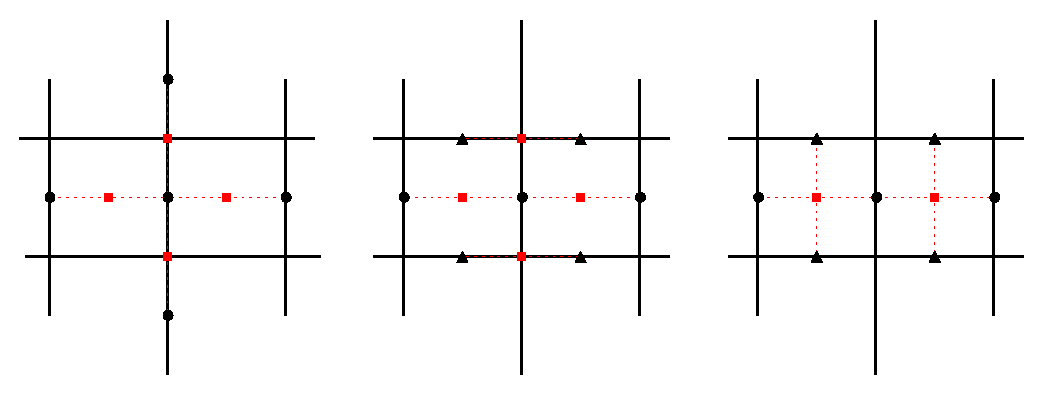
\includegraphics[width=5.25in]{viscOp}
\caption{The stencils for the $x$-component of (Left) $\nabla\cdot\beta\nabla\vb$, (Middle) 
$\nabla\cdot\beta(\nabla\vb)^T$, and (Right) $\nabla\cdot[\mathcal{I}(\gamma-\frac{2}{3}\beta)(\nabla\cdot\vb)]$.  
The black circles indicate locations of $u$.
The black triangles indicate locations of $v$.
The red dots indicate the location of the $\beta$ and the gradients of velocity.}\label{fig:viscOp}
\end{figure}
%%%%%%%%%%%%%%%%%%%%%%%%%%%%%%%%%
%%%%%%%%%%%%%%%%%%%%%%%%%%%%%%%%%
\begin{figure}[tb]
\centering
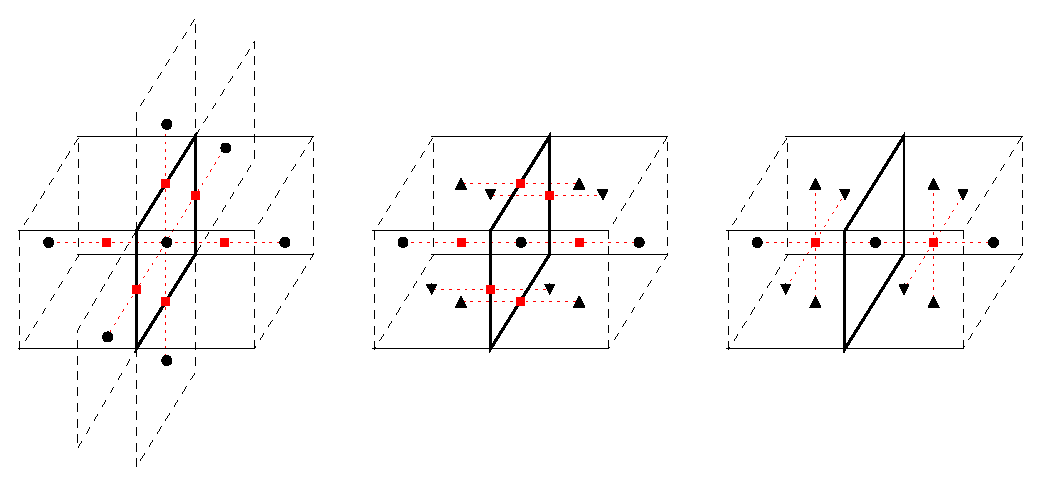
\includegraphics[width=5.25in]{viscOp_3d}
\caption{The stencils for the $x$-component of (Left) $\nabla\cdot\beta\nabla\vb$, (Middle) 
$\nabla\cdot\beta(\nabla\vb)^T$, and (Right) $\nabla\cdot[\mathcal{I}(\gamma-\frac{2}{3}\beta)(\nabla\cdot\vb)]$.  
The black circles indicate locations of $u$.
The black triangles indicate locations of $v$ and $w$.
The red dots indicate the location of the $\beta$ and the gradients of velocity.}\label{fig:viscOp_3d}
\end{figure}
%%%%%%%%%%%%%%%%%%%%%%%%%%%%%%%%%
For velocities, it is helpful to first consider the stencils 
for the viscous operators, as illustrated
in Figures \ref{fig:viscOp} and \ref{fig:viscOp_3d} for two and three dimensions.
There are a few key design principles to keep in mind:\\
\begin{itemize}
\item The viscous operator for faces {\it on} any physical boundary must
evaluate to zero, so it does not matter what value is stored for the normal component
of velocity in the ghost face immediately outside of the valid region, unless you 
are concerned 
about possible intermediate {\tt NaN} states that will later be overwritten.\\
\item The value of the normal velocity {\it on} the boundary {\it does} matter, since it
enters the stencil for the first interior normal velocity face and stencils for the
transverse velocity near the boundary.\\
\item The value of transverse velocities in ghost faces behind physical boundaries
{\it does} matter, since it enters the stencil for the interior transverse face.
We make sure to fill these using the appropriate physical boundary condition.\\
\item When setting normal velocities on physical boundaries, we don't have to worry
about corner ghost faces outside of the domain.  Those only matter if we are periodic 
in the transverse
direction, in which case the call to {\tt multifab\_fill\_boundary} should take care of
these periodic values.\\
\item When setting transverse velocity ghost faces behind physical boundaries, we do
not have to worry about ghost faces that are outside the valid region with respect
to the problem domain in the transverse direction.  Those only matter if we are 
periodic in the transverse direction, in which case the call to {\tt multifab\_fill\_boundary}
should take care of these periodic values.\\
\item Unlike the case for scalars, here the values of velocity in ghost cells represent
the value extrapolated to that point (for tangential velocities), or the value {\it on}
the boundary (for normal velocities).\\
\end{itemize}

We carry around several auxiliary multifabs that store the Dirichlet values 
for velocity on the
boundary, whether they are homogeneous or inhomogeneous.  To deal with normal 
velocities, the multifab {\tt vel\_bc\_n(nlevs,dm)}
stores the actual Dirichlet value.  The $(n,d)^{\rm th}$ element is a face-centered
multifab for refinement level $n$ in direction $d$ and does not require ghost cells.
The boundary face itself stores the Dirichlet value.\\

To deal with transverse velocities, the multifab {\tt vel\_bc\_t(nlevs,X)} stores
either the Dirichlet or Neumann value (depending on the boundary type), for both 
inhomogeneous and homogeneous cases.  In 2D, X=2,
and in 3D, X=6.  In 2D, the multifabs are each nodal and the components represent:\\
\begin{enumerate}
\item The y-velocity bc on x-faces.
\item The x-velocity bc on y-faces.\\
\end{enumerate}

In 3D, the multifabs are edge-based (i.e., nodal in 2 directions)
and the components represent:\\
\begin{enumerate}
\item The y-velocity bc on x-faces (thus is nodal in y and x).
\item The z-velocity bc on x-faces (thus is nodal in z and x).
\item The x-velocity bc on y-faces (thus is nodal in x and y).
\item The z-velocity bc on y-faces (thus is nodal in z and y).
\item The x-velocity bc on z-faces (thus is nodal in x and z).
\item The y-velocity bc on z-faces (thus is nodal in y and z).\\
\end{enumerate}

Note that none of these multifabs require any ghost cells.\\

\subsection{Implementation}

To fill {\tt vel\_bc\_n} and {\tt vel\_bc\_t} we call the subroutine,
{\tt set\_inhomogeneous\_vel\_bcs}.  This routine loops over domain boundary
faces, and if the domain boundary is a physical boundary, it uses the
function {\tt inhomogeneous\_bc\_val\_Xd} to fill {\tt vel\_bc\_n} and 
{\tt vel\_bc\_t}.\\

We have two subroutines that fill velocity domain boundary and ghost cells based
on the values in {\tt vel\_bc\_n} and {\tt vel\_bc\_t}.

Each of these take in {\tt vel\_bc\_n} or {\tt vel\_bc\_t} as
an optional multifab argument that represents the prescribed Dirichlet
or Neumann value on the boundary.  
The subroutine {\tt multifab\_physbc\_domainvel} sets the 
value for faces on the boundary and can take {\tt vel\_bc\_n} as an optional input.
The subroutine {\tt multifab\_physbc\_macvel}
sets the transverse velocity ghost faces behind the physical boundary and
can take {\tt vel\_bc\_t} as an optional input.
If no multifab is passed in, it is assumed that the boundary conditions
are homogeneous.\\

For {\tt multifab\_physbc\_macvel}, the optional multifab that gets passed in
must be nodal in exactly 2 directions.
We use the domain value to represent
the Dirichlet or Neumann value, and then depending on the boundary conditions, the 
appropriate stencil is used to fill in the ghost value.
The stencil for transverse velocities is a two-point stencil involving the
interior value and the Dirichlet or Neumann boundary value.\\

The subroutine {\tt set\_inhomogeneous\_vel\_bcs} sets the Dirichlet or
Neumann condition, $f$, for normal and transverse velocities.  For the case of 
reservoir boundary conditions, it sets $f=0$ and relies on other subroutines 
to update the normal velocity boundary condition as the fluxes for the concentrations
are built up.\\

The subroutine {\tt modify\_traction\_bcs} is a standalone subroutine that
modifies the traction boundary condition by subtracting off the 
$\partial v_n/\partial\tau$ term for the Neumann conditions
on $v_{\tau}$.  This only matters if the normal velocity
changes as a function of the transverse velocity of interest.  This subroutine
should only be called after calling the inhomogeneous version of 
{\tt multifab\_physbc\_domainvel}.

\subsection{Calling Sequence}
WORK IN PROGRESS... NOT CORRECT YET... Since in the GMRES solve at the end of the
time step we use new-time stochastic fluxes the sequencing here gets tricky.\\

A typical calling sequence for a low Mach number algorithm for a given time
step should look something like:
\begin{enumerate}
\item Assume we start with $\rho$ and $c$ in the valid region, as well as
velocities everywhere in the valid region {\it except} on the boundary.
\item Call {\tt multifab\_fill\_boundary} to fill ghost cells for $\rho$ and
$c$, noting that the ghost value represent the value on the boundary.
\item Compute transport coefficients that are a function of $\rho$ and $c$ by
looping over valid {\it and} ghost regions.
\item Call {\tt set\_inhomogeneous\_vel\_bcs} to fill the bc multifabs,
{\tt vel\_bc\_n} and {\tt vel\_bc\_t}.
\item Compute the diffusive and stochastic $\rho c$ fluxes, making sure to update
{\tt vel\_bc\_n} for the reservoir case.
\item Call the inhomogeneous versions of {\tt multifab\_physbc\_macvel} and
{\tt multifab\_physbc\_domainvel}.
\end{enumerate}

\subsection{GMRES Boundary Conditions}
The GMRES solver assumes homogeneous boundary conditions,
so we use a residual correction technique to convert the problem to one
with homogeneous boundary conditions of the same type (Neumann or Dirichlet):
\begin{equation}
\Ab_H\xb = \bb - \Ab\xb_H.
\end{equation}
Here, $\Ab_H$ is the same operator as $\Ab$, but with homogeneous boundary conditions
of the same type.
The vector $\xb_H$ is a vector with zeros in all valid cells (but possibly
non-zero values on the boundary and in the ghost cells, depending on the 
boundary conditions).
By solving this system for $\xb$, we arrive at the same answer as solving the
inhomogeneous problem, $\Ab\xb=\bb$.\\

It is also important to note that we are solving a ``delta'' formulation for
$(\deltab\vb,\delta p)$.  This means we have to be careful when supplying
a boundary condition to the subroutine that converts the problem to a homogeneous
problem, in that for time-dependent boundary conditions (such as reservoirs), we
must supply the {\it change} in the velocity boundary condition as compared to
the boundary condition at $t^n$, rather than the final velocity boundary 
condition itself.

\end{document}
